\section{Introduction}
\label{sec:intro}

Electric vertical-take-off-and-landing (eVTOL) aircraft are increasingly
positioned as a near-term airport-shuttle service, connecting major
international airports to downtown cores, rail hubs, and remote
parking facilities \citep{vascik2019,bulusu2021}. Most operational
analyses treat the airport-side of that connection as a routine
low-altitude routing problem in urban airspace
\citep{kleinbekman2020,pang2022}. Airport airspace, however, is not flat
low-altitude airspace. It is partitioned by ICAO Annex~14 obstacle
limitation surfaces (OLS) -- the approach, takeoff-climb, transitional,
inner-horizontal, conical, runway-strip, runway-end-safety-area, and
obstacle-free-zone surfaces -- whose purpose is to protect conventional
fixed-wing operations on the active runway configuration~\citep{icao_annex14}.
These surfaces \emph{shift} with the active runway configuration, with the
prevailing wind, and with arrival/departure flow.

A safety-conscious eVTOL shuttle planner therefore faces a dilemma. If it
respects Annex~14 \emph{statically} -- that is, without knowing which runway
is active -- it has no choice but to pessimistically close the protected
volume above \emph{both} parallel-runway corridors at every parallel-runway
airport. Empirically this leaves only a small fraction of plausible
vertiport pairs reachable. If it respects only the immediate protection of
the currently active runway, it requires operational data feeds (typically
ADS-B and METAR) that have hitherto been treated as out of scope for the
corridor-planning step. The literature does not, to our knowledge, quantify
the gap between these two options on real airport data.

\paragraph{Contributions.}
We close this gap with \textbf{DREAM} -- a Dynamic Runway-configuration-aware
Envelope for eVTOL Airport Mobility -- and show on real
August-2024 LAX and SFO operational data that runway-configuration awareness
recovers $2.0\times$~LAX and $4.5\times$~SFO of the vertiport-pair feasibility
that a static Annex-14-only baseline forbids. Concretely:
\begin{enumerate}
    \item \textbf{Machine-readable Annex~14.} We encode the nine Annex~14
    surface families as 3-D prisms on each airport's east-north-up grid and
    reduce them to a signed-distance field that supports
    constant-time \texttt{is\_clear} and \texttt{clearance\_m} queries
    (\cref{sec:method-sdf}).
    \item \textbf{ADS-B-driven runway configuration.} We infer the active
    arrivals and departures per 15-minute slice from real fixed-wing ADS-B
    with a METAR cross-check (\cref{sec:method-config}). On real data the
    cross-check passes on $28/29 = 96.6\,\%$ of scoreable slices across our
    ten airport-days.
    \item \textbf{DREAM dynamic envelope.} We compose the static both-sides
    closed Annex~14 mask $\Astatic$ with a time-varying closure $\Cdyn$
    driven by $(\Rt,\Wt,\Ft)$ -- runway configuration, weather and
    fixed-wing flow -- to produce $\Edyn = \Astatic \setminus \Cdyn$, the
    space an eVTOL corridor planner may use at time~$t$
    (\cref{sec:method-envelope}). This is the operational contribution.
    \item \textbf{Counterfactual-injection risk field.} We sample candidate
    eVTOL segments inside $\Astatic \cap \Edyn$ and label each by a
    deterministic geometric and kinematic test against \emph{real}
    fixed-wing ADS-B trajectories (\cref{sec:method-risk}). We then train
    logistic-regression, random-forest, gradient-boosted and multi-layer
    perceptron classifiers, and wrap them in split-conformal prediction.
    Under a temporal hold-out (four-day train, one-day test), gradient
    boosting reaches AUROC = $0.716$ at SFO with conformal coverage = $0.912$.
    \item \textbf{Envelope-constrained planning and joint assessment.} We
    plan corridors with an $A^\star$ that respects $\Edyn$ and a five-term
    cost over time, energy, risk, noise and capacity-impact
    (\cref{sec:method-planner}), and assess safety, capacity, and
    accessibility on the resulting corridors
    (\cref{sec:lax,sec:sfo}).
    \item \textbf{Counterfactual injection as operational honesty.} No
    large-scale commercial eVTOL service exists at LAX or SFO. We argue
    counterfactual injection into the real fixed-wing operational scene,
    with deterministic labels rather than surrogate-model labels, is the
    methodologically honest framing for empirical analysis at the current
    industry stage (\cref{sec:method-counterfactual,sec:discussion}).
    \item \textbf{Cross-airport replication.} We re-run the full pipeline on
    SFO without re-tuning weights and obtain the same $B0 < B1$, $B3 \supsetneq B2$
    ordering, with the SFO advantage \emph{larger} than LAX's because SFO's
    lower base traffic exposes the over-conservatism of static both-sides
    protection more sharply (\cref{sec:sfo}).
\end{enumerate}

\paragraph{Headline number.}
\Cref{fig:hero} shows the central result. At LAX, runway-configuration
awareness lifts vertiport-pair feasibility from $33\,\%$ to $65\,\%$; at SFO,
from $17\,\%$ to $75\,\%$. The cost of safety, in path-length terms, is
$\leq 20 \%$ on the pairs both baselines find. The operational implication is
that airport-aware UAM planning needs Annex~14 \emph{and} the operational
awareness; neither alone is sufficient.

% --- Hero figure (Fig 1) -------------------------------------------------
\begin{figure*}[t]
    \centering
    \begin{minipage}[t]{0.49\linewidth}
        \centering
        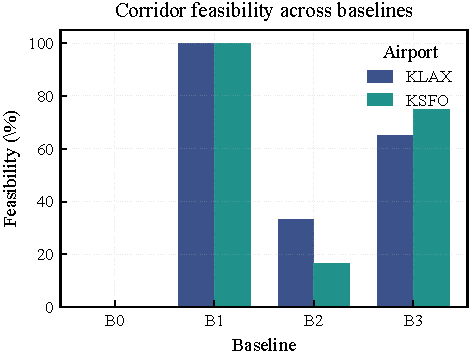
\includegraphics[width=\linewidth]{../figures/paper/fig_feasibility_by_baseline.pdf}
        \subcaption{Per-baseline corridor feasibility.}
        \label{fig:feas-bar}
    \end{minipage}\hfill
    \begin{minipage}[t]{0.49\linewidth}
        \centering
        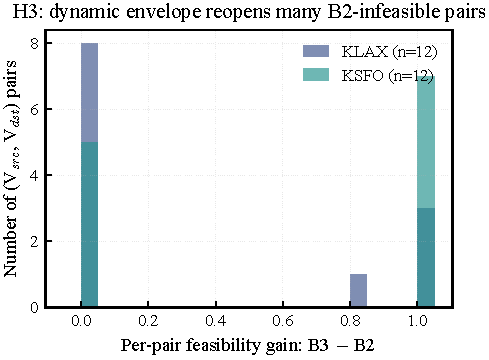
\includegraphics[width=\linewidth]{../figures/paper/fig_h3_b2_vs_b3.pdf}
        \subcaption{Per-pair $B_3 - B_2$ feasibility gain.}
        \label{fig:h3-hist}
    \end{minipage}
    \caption{\textbf{Headline result.} The runway-configuration-aware dynamic
        envelope ($B_3$) recovers $\boldsymbol{2.0\times}$ of LAX and
        $\boldsymbol{4.5\times}$ of SFO vertiport-pair feasibility that the
        static Annex~14 both-sides-closed baseline ($B_2$) pessimistically
        forbids, on real ADS-B from five Aug-2024 Fridays per airport.}
    \label{fig:hero}
\end{figure*}

\paragraph{Paper organisation.}
\Cref{sec:related} situates DREAM against eVTOL/UAM corridor planning,
airport obstacle protection (ICAO/FAA/EASA), ADS-B-based airport analytics, and
counterfactual/conformal risk modelling. \Cref{sec:method} describes the five
DREAM stages in turn. \Cref{sec:data} documents the eight real data sources
and the operational scope of our study. \Cref{sec:lax} reports the LAX case
study; \cref{sec:sfo} the SFO external validation; \cref{sec:discussion} the
discussion and limitations; \cref{sec:conclusion} concludes.
